\label{section:case-studies:results-and-discussion}
%
\begin{figure}
  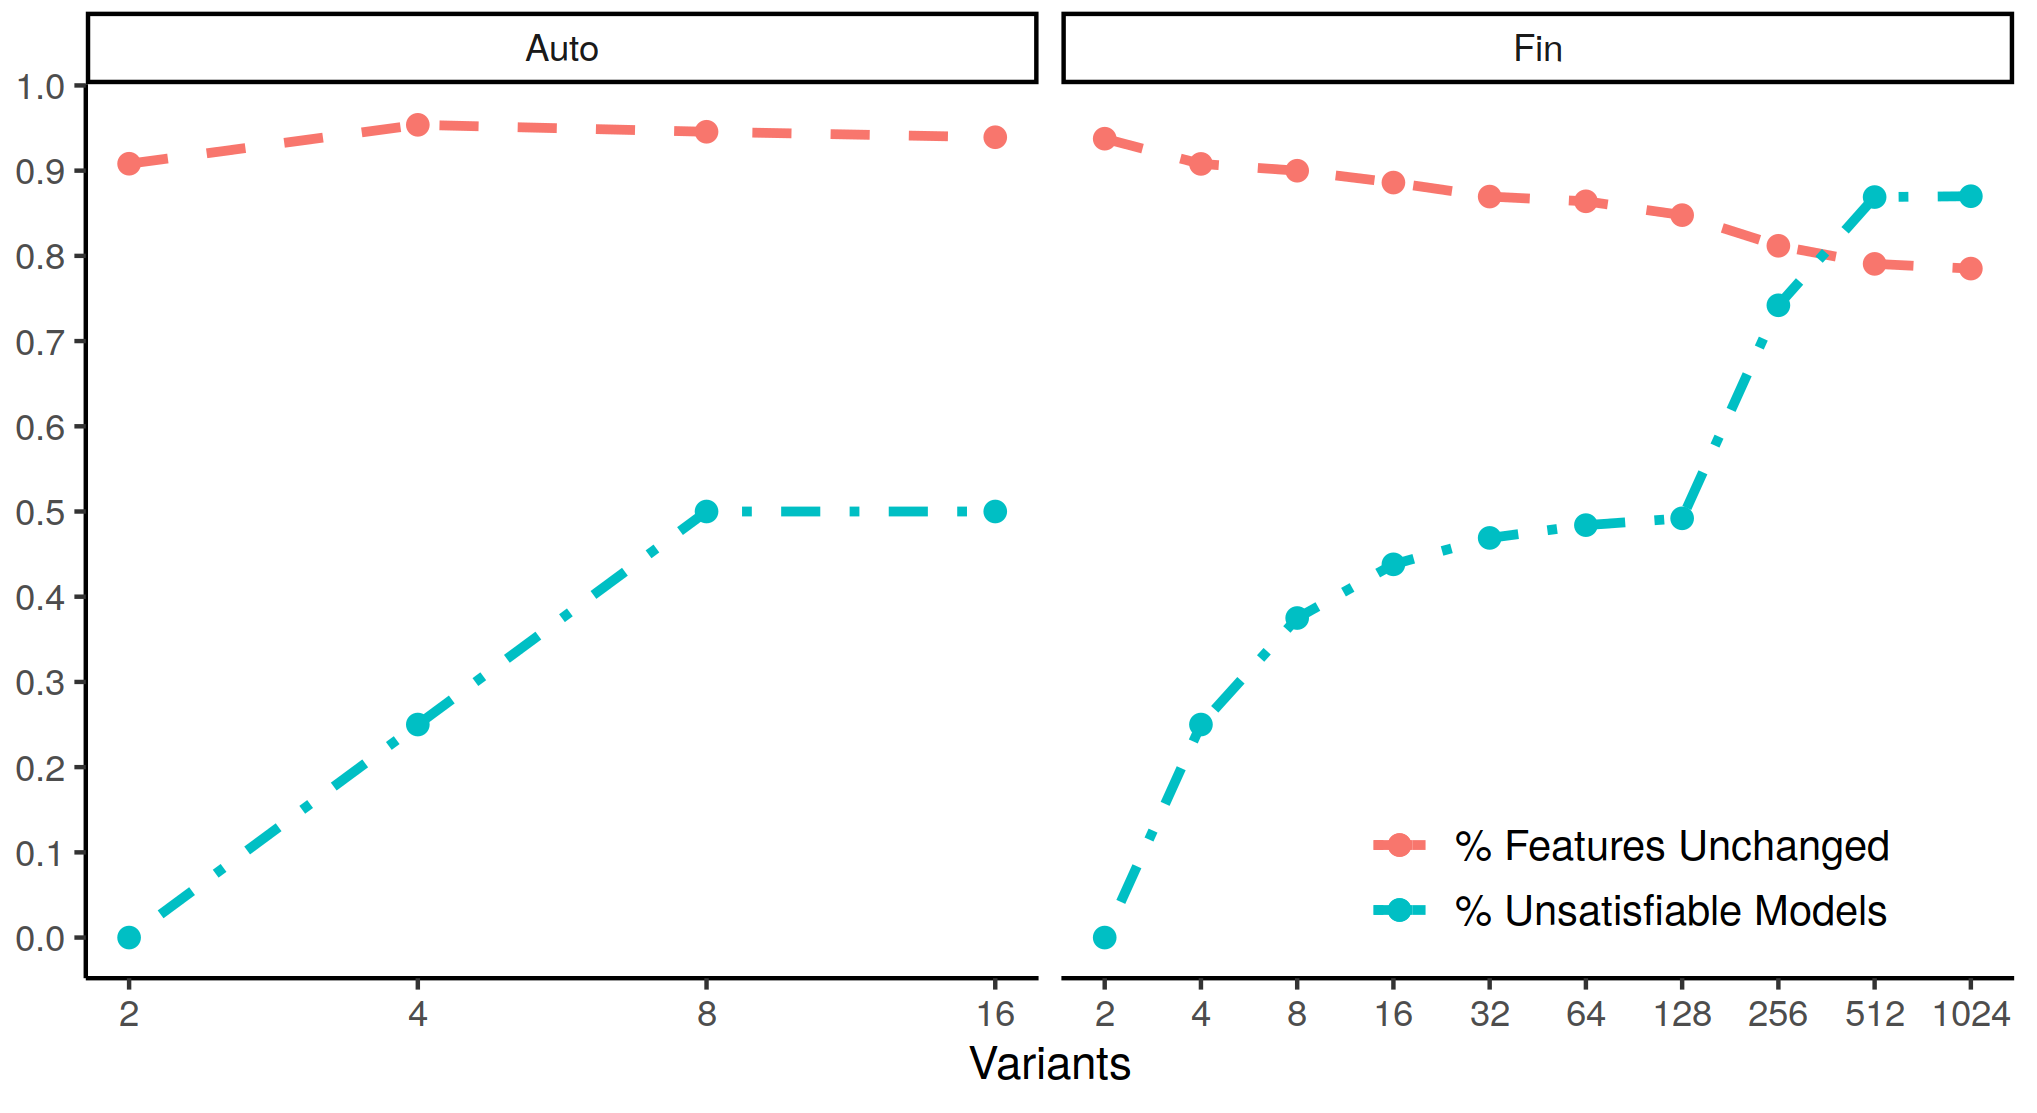
\includegraphics[width=0.95\textwidth]{Plots/VModel}
  \caption{Ratio of models found to be unsatisfiable.}%
  \label{res:vmodels}
\end{figure}
%
The datasets yielded dissimilar query formulas: the \auto{} query formula
consisted of 4,212 choice terms (not including terms in a choice's
alternatives), and 26,808 plain terms. In contrast, \fin{} had 3,809 choice
terms, and 1,441 plain terms. Thus \fin{} had larger changes between product
line versions. \autoref{res:vmodels} shows the ratio of unsatisfiable models to
total plain models, and the ratio of constant features for each product line
version (represented by variant count). For both datasets the number of
satisfiable models decreased as new versions were considered, and the majority
of features in each model never flipped from their initialized value \fls{} to
\tru{}. Thus, the variational model is likely a compressed version of the set
of plain models. Compression metrics were not calculated as this is an
orthogonal concern to the performance of variational satisfiability solving.

Variational models permit product analyses without a \ac{sat} solver.
\autoref{res:vmodels} shows such a purely syntactic analysis: counting
disjuncted clauses in the variational model as a representation of satisfiable
plain models. We believe post-hoc analyses such as this may be useful to feature
modelers as they direct attention to impactful versions of the feature model.
For example, the change from $V_{7}$ to $V_{8}$ (128 to 256 Variants) of \fin{}
clearly constrained the feature model as the number of unsatisfiable models
increased from 50\% to 80\%.

The experiment required 7 days, 6 hours, and 21 minutes to complete. Due to the
amount of time required to generate the data, we limited the number of raw
measurements to 3. Thus, each data point presented in our results is a
bootstrapped average of 3 raw measurements.

\subsection{RQ1: Performance of Variational Solving as Variation Scales}

\begin{figure}
  \centering
  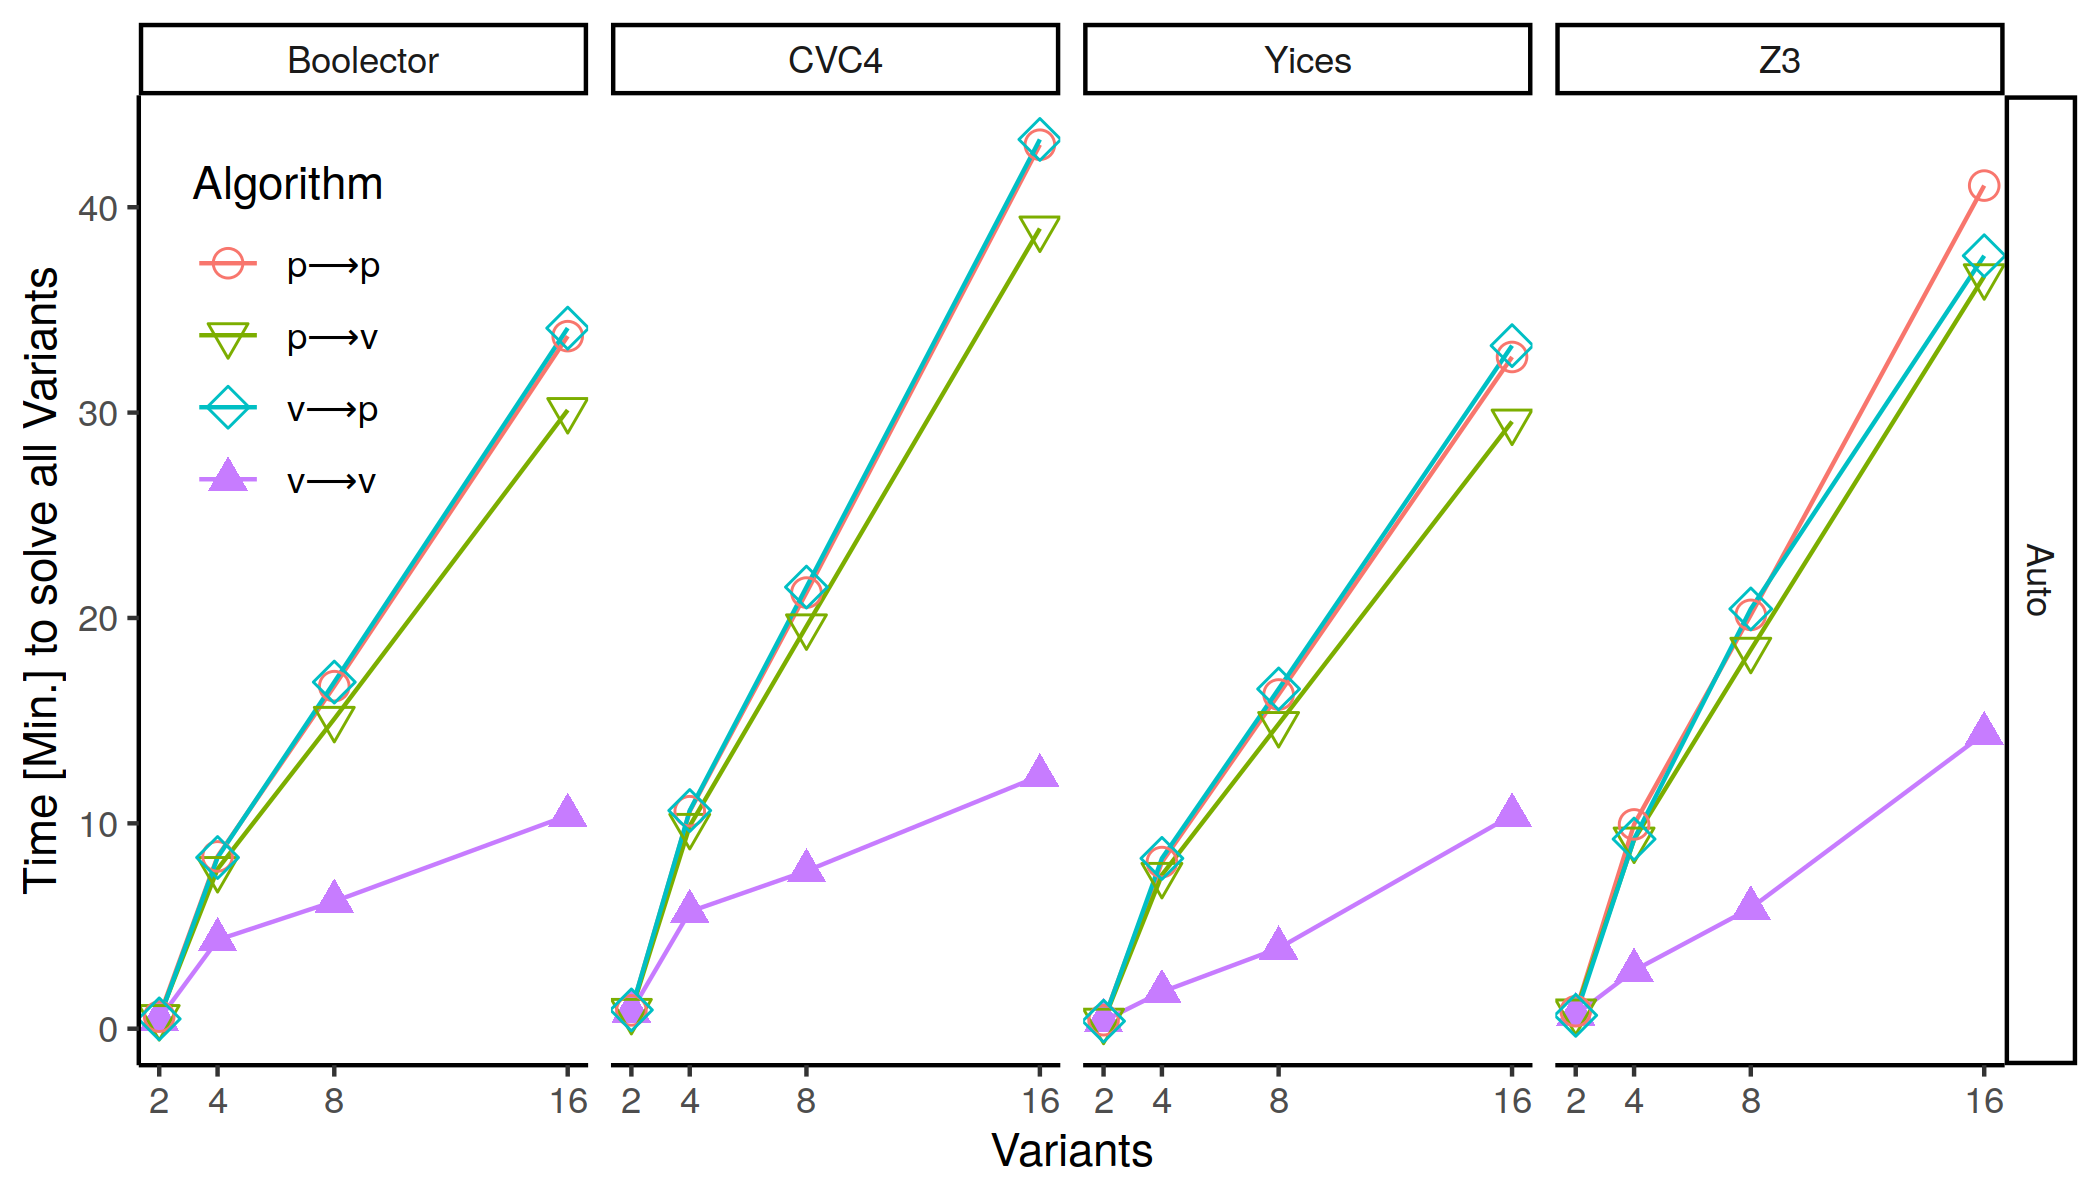
\includegraphics[width=0.95\textwidth]{Plots/RQ1_Auto}
  \caption{(Auto) RQ1: performance as variants increase per base solver. \vTov{}
    shows a speedup of 2.8--3.5x for the \auto{} dataset depending on base
    solver.}%
  \label{res:rq1:auto}
\end{figure}
%
\begin{figure}[h]
  \centering
  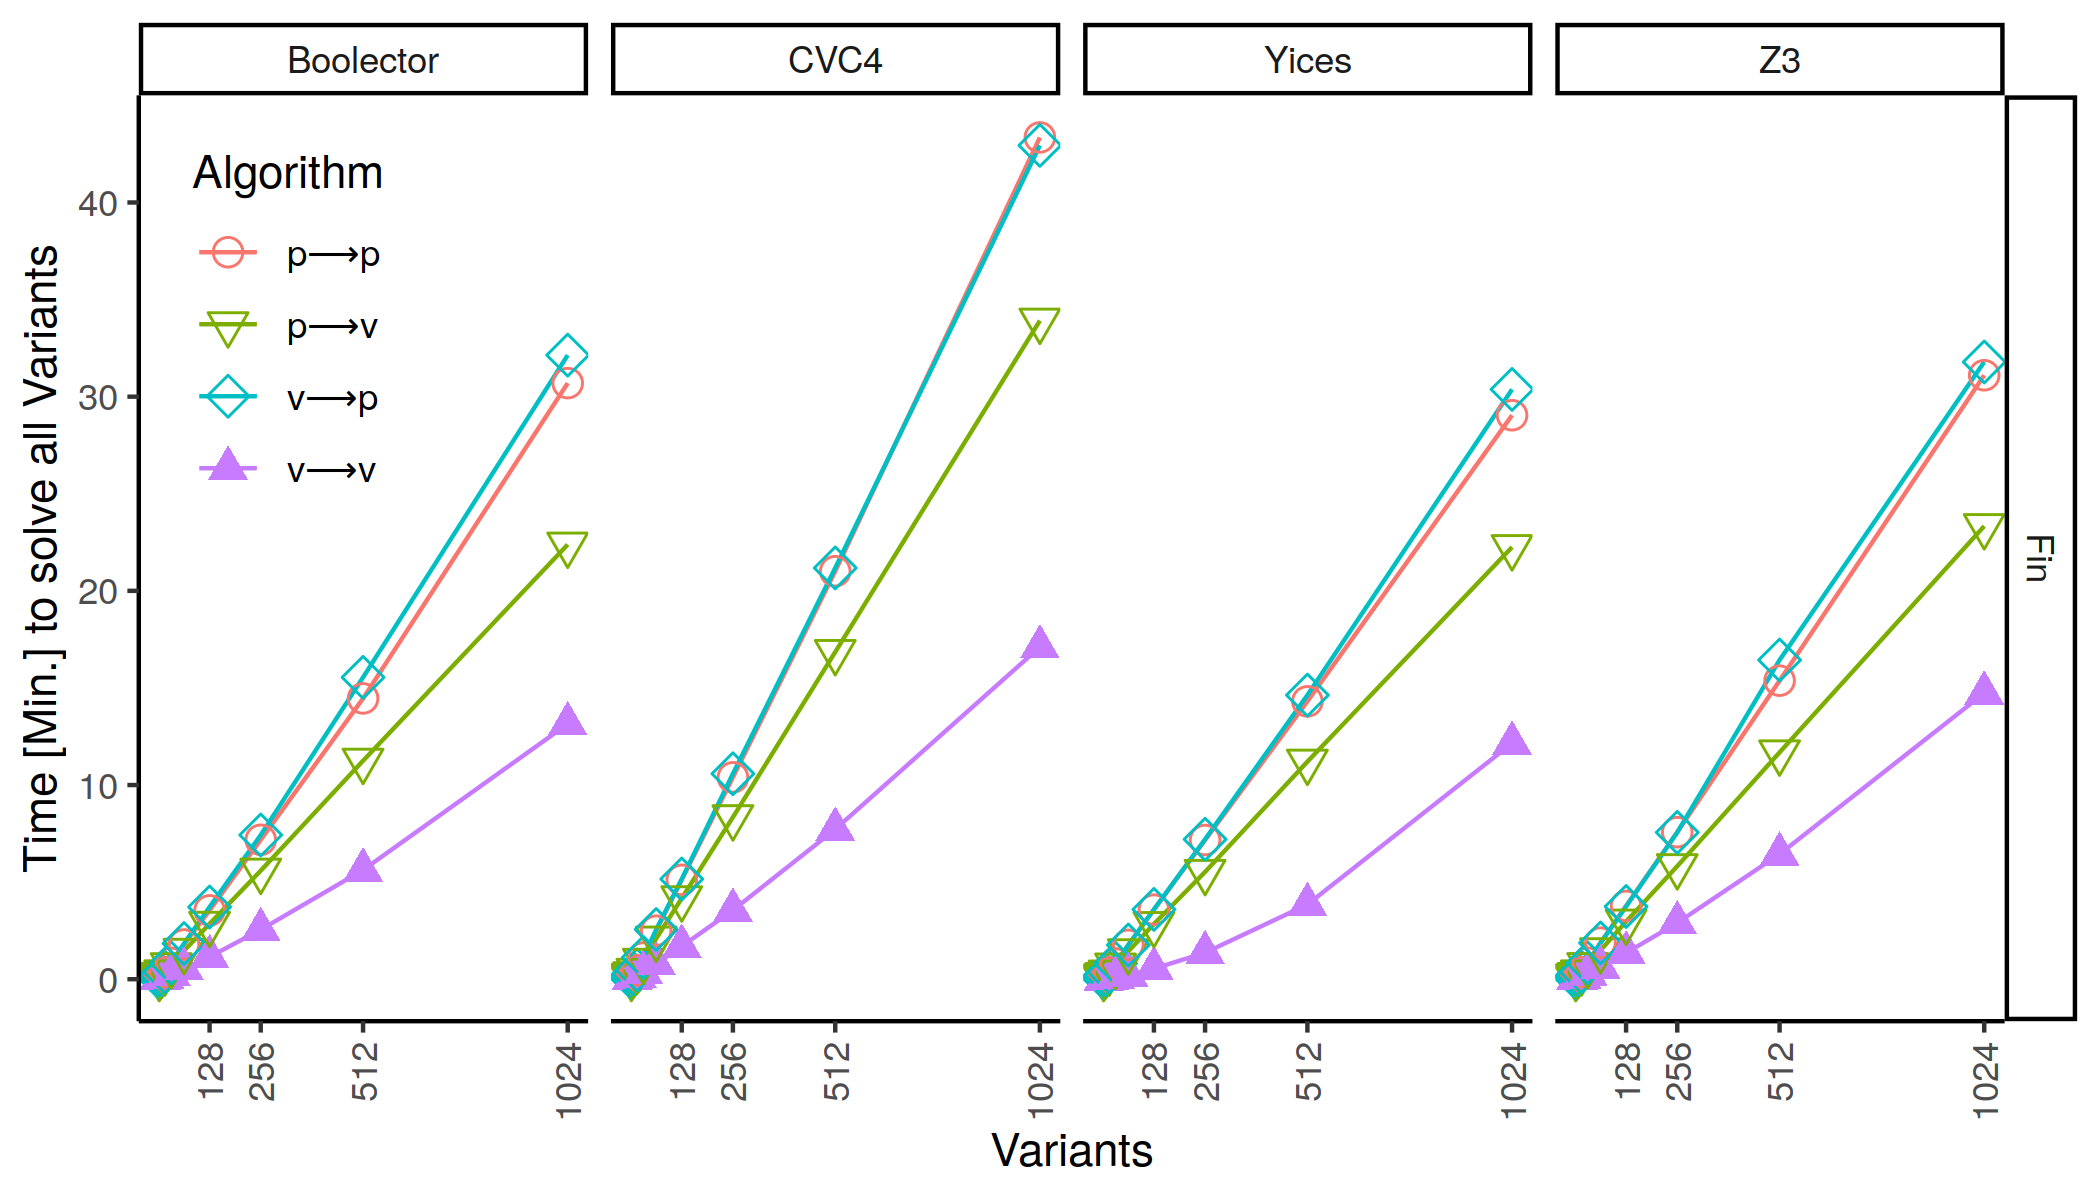
\includegraphics[width=0.95\textwidth]{Plots/RQ1_Fin}
  \caption{(Financial) RQ1: performance as variants increase per base solver. \vTov{}
    shows a speedup of 2.4--3.2x for the \fin{} dataset depending on the base
    solver. Overlapping x-axis labels elided.}%
  \label{res:rq1:fin}
\end{figure}

\begin{table}
  \begin{subtable}[t]{0.45\textwidth}
    \centering
    \begin{tabular}{c || c | c | c | c}
      DataSet    & Boolector & CVC4 & Yices & Z3 \\
      \hline
      \auto{}    & 3.29      & 3.51 & 3.20  & 2.62 \\
      \fin{}     & 2.44      & 2.51 & 2.50  & 2.16 \\
    \end{tabular}
    \caption{Speedup by solver for the maximum variant case; 16 for \auto{},
      1024 for \fin{}.}%
    \label{tab:rq1:speedup}
  \end{subtable}
  \hfill
  \begin{subtable}[t]{0.45\textwidth}
    \centering
    \begin{tabular}{ c | c | c | c}
      Boolector & CVC4 & Yices & Z3 \\
      \hline
       623.0    & 738.6 & 623.7 & 862.0 \\
       788.8     & 1026.6 & 729.2  & 884.2 \\
    \end{tabular}
    \caption{Time [s] to solve with \vTov{} by solver.}%
    \label{tab:rq1:comparison}
  \end{subtable}
  \caption{Time to solve and speedup of most variational case by solver.}%
  \label{tab:rq1}
\end{table}

The \vsat{} tool outperforms other algorithms as the count of variants to solve
increases for every base solver. \autoref{res:rq1:auto} shows the time to solve
the query formula as variants increase from 2 to 16 for the \auto{} dataset for
each solver. Similarly \autoref{res:rq1:fin} shows time to solve by base solver
for the \fin{} dataset.

For the \auto{} dataset, variational solving is faster with an average speedup
of 2.60x. For the most variational case (16 variants) the greatest speedup was
found to be 3.5x with cvc4. The \fin{} dataset shows an average speedup of
4.70x~\footnote{Due to extreme outliers (10x--15.1x speedup) from yices when
  solving 2--32 variants.}. For the most variational case (1024 variants), cvc4
also showed the greatest speedup at 2.51x. We find that \vTov{} is statistically
different from every other algorithm with p-values of $2.77\times 10^{-4}$
(\vTop{}), $1.06\times 10^{-2}$ (\pTop{}), and $1.92\times 10^{-2}$ (\pTov{})
for \auto{} and $1.62\times 10^{-5}$ (\vTop{}), $1.92\times 10^{-5}$ (\pTop{}),
and $1.70\times 10^{-4}$ (\pTov{}) for \fin{}.

\vsat{} outperforms the other algorithms because the variational core caches
plain terms, thereby preventing the re-evaluation of these terms for each
variant. By this data, we observed a constant factor speedup. Thus, variational
solving still grows linearly in the number of variants being solved.


\subsection{RQ2: Performance Impact of Base Solver}
%
From \resQ{1} we determined that \vTov{} is faster than the baseline algorithms
and that the difference is statistically significant. We observe from
\autoref{res:rq1:auto} and \autoref{res:rq1:fin} that the \vTov{} algorithm is
robust across every tested base solver and \vTov{} produced reasonable results
with each base solver.
%
We summarize our results in \autoref{tab:rq1}. Notable yices was consistently
the most performent base solver for all algorithms and all test cases. For
\vTov{} yices demonstrates not only a high degree of speedup but also a
reduction of 238.3 seconds, and 132.8 seconds, in run time from z3 for the
most variational case of \auto{} and \fin{}. Thus, yices is an attractive
target for the base solver of future prototype variational \ac{sat} solvers.

Cvc4 is also noteworthy; cvc4 benefited the most from \vTov{} for both
datasets with a speedup 3.51x (\auto{}) and 2.51 (\fin{}). The cvc4 case is
interesting as it implies that a base solver which shows poor performance with
in the typical use case (\vTop{}; \ac{sat} calls occur in an incremental
context, and solver is kept alive) may greatly benefit from the variational
solving algorithm we've presented. Although the exact reasons behind this
behavior will be particular to the base solver, these results imply that our
use case (\ie{}, heavily exercising the incremental code paths) is peculiar
and thus selecting a solver based on only its typical performance may not be
representative of its performance in this use case.

\subsection{RQ3: Performance Impact of Plain Terms}
We hypothesize that the ratio of plain terms to total terms should increase the
variational solver's performance. Specifically, we hypothesize that as sharing
grows, the query formula's variational core is further reduced. We observe this
behavior using the z3 data in \autoref{res:speedup}. Both \vTov{} and \pTop{}
showed a statistically significant fit to a linear model. Furthermore, only
\vTov{} was found to be statistically different from \pTop{} and \pTov{} with
p-values of $6.95\times 10^{-3}$ and $4.44\times 10^{-6}$ thus confirming that
sharing positively correlates to speedups for variational solving in these
datasets.

This result is evidence that a dataset's sharing ratio is an important factor in
the performance of a variational \ac{sat} solver, as we hypothesized. When the
sharing ratio is high, the reduction engine produces a smaller variational core.
With a smaller variational core, more reuse of plain terms occurs and thus
computational time is saved in the base solver. Hence, an avenue of future work
is to leverage the laws of the variational logic to automatically refactor input
formulas to increase sharing. The consequences of this observation will be
particular to the application domain. For software product lines this means that
any method to increase sharing between product line versions or the
representative \ac{sat} problems is desirable; this may be smaller changes with
respect to the entire feature model, more frequent snapshots of the feature
model, or syntactic manipulations to mitigate the occurrence of new features.

\begin{figure}
  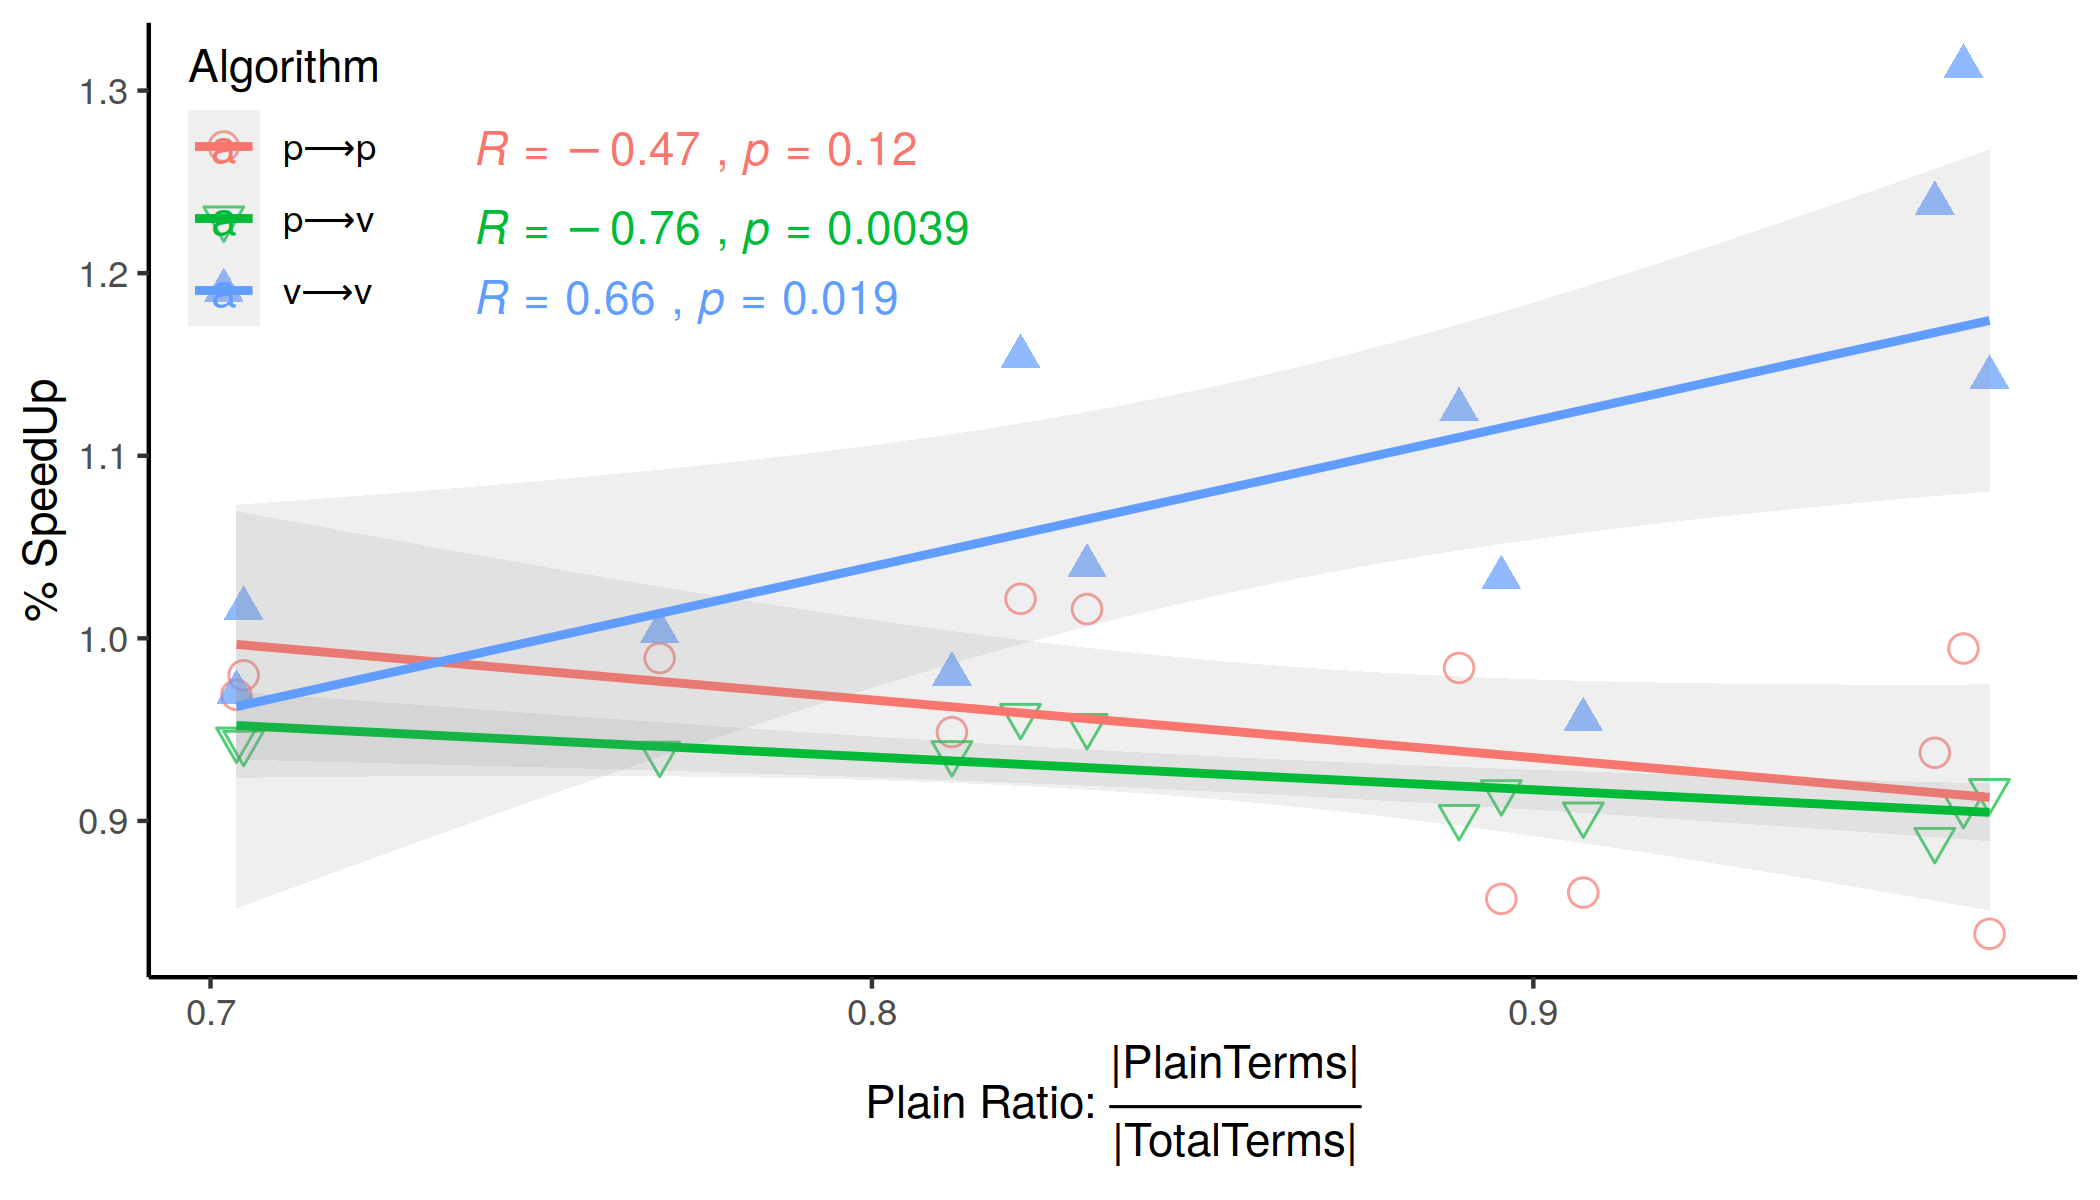
\includegraphics[width=0.95\textwidth]{Plots/RQ3}
  \caption{RQ3: performance as a function of plain ratio. We observe that
    sharing positively correlates to speedup only for \vTov{}, where $\texttt{\%
      SpeedUp} = \frac{{\text{Algorithm}}}{{\text{\vTop{}}}}$.}%
  \label{res:speedup}
\end{figure}

\subsection{RQ4: Overhead of a Plain Query on \vsat{}}
%
\begin{figure}
  \begin{subfigure}[t]{\textwidth}
    \centering
    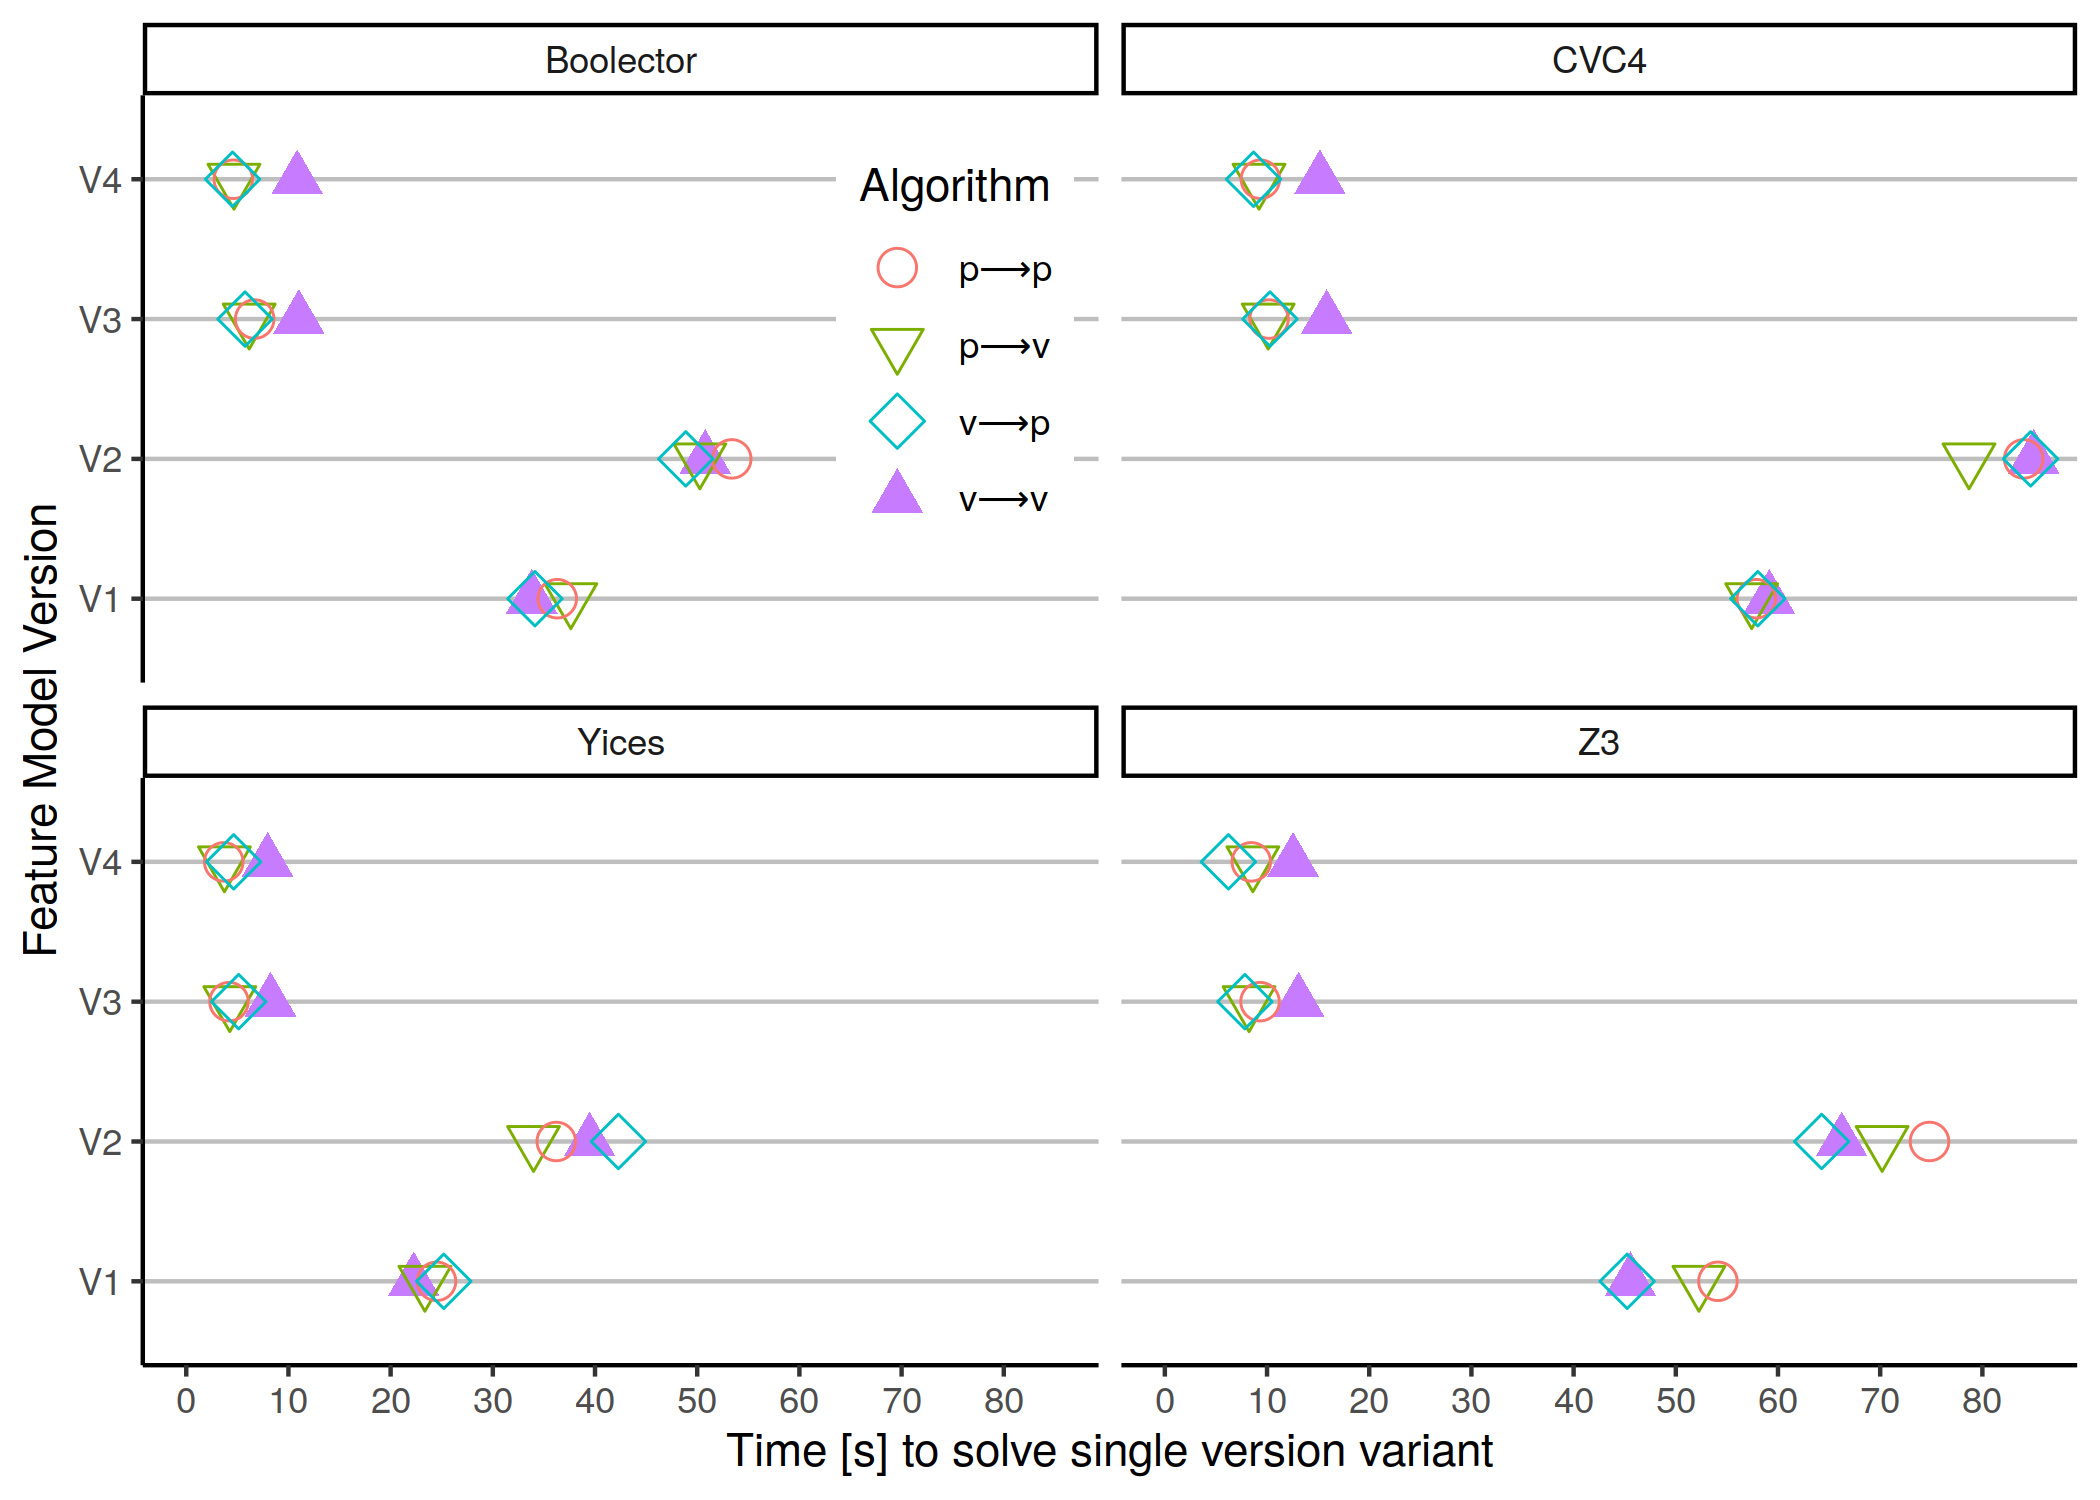
\includegraphics[width=0.95\textwidth]{Plots/RQ4_Auto}
    \caption{(Auto) RQ4: Overhead of \vTov{} on plain formulas. We observe that
      \vTov{} incurs an average slowdown of 9\% for \auto{}, when
      solving a version variant.}%
    \label{res:overhead:auto}
  \end{subfigure}
~
  \begin{subfigure}[t]{\textwidth}
    \centering
    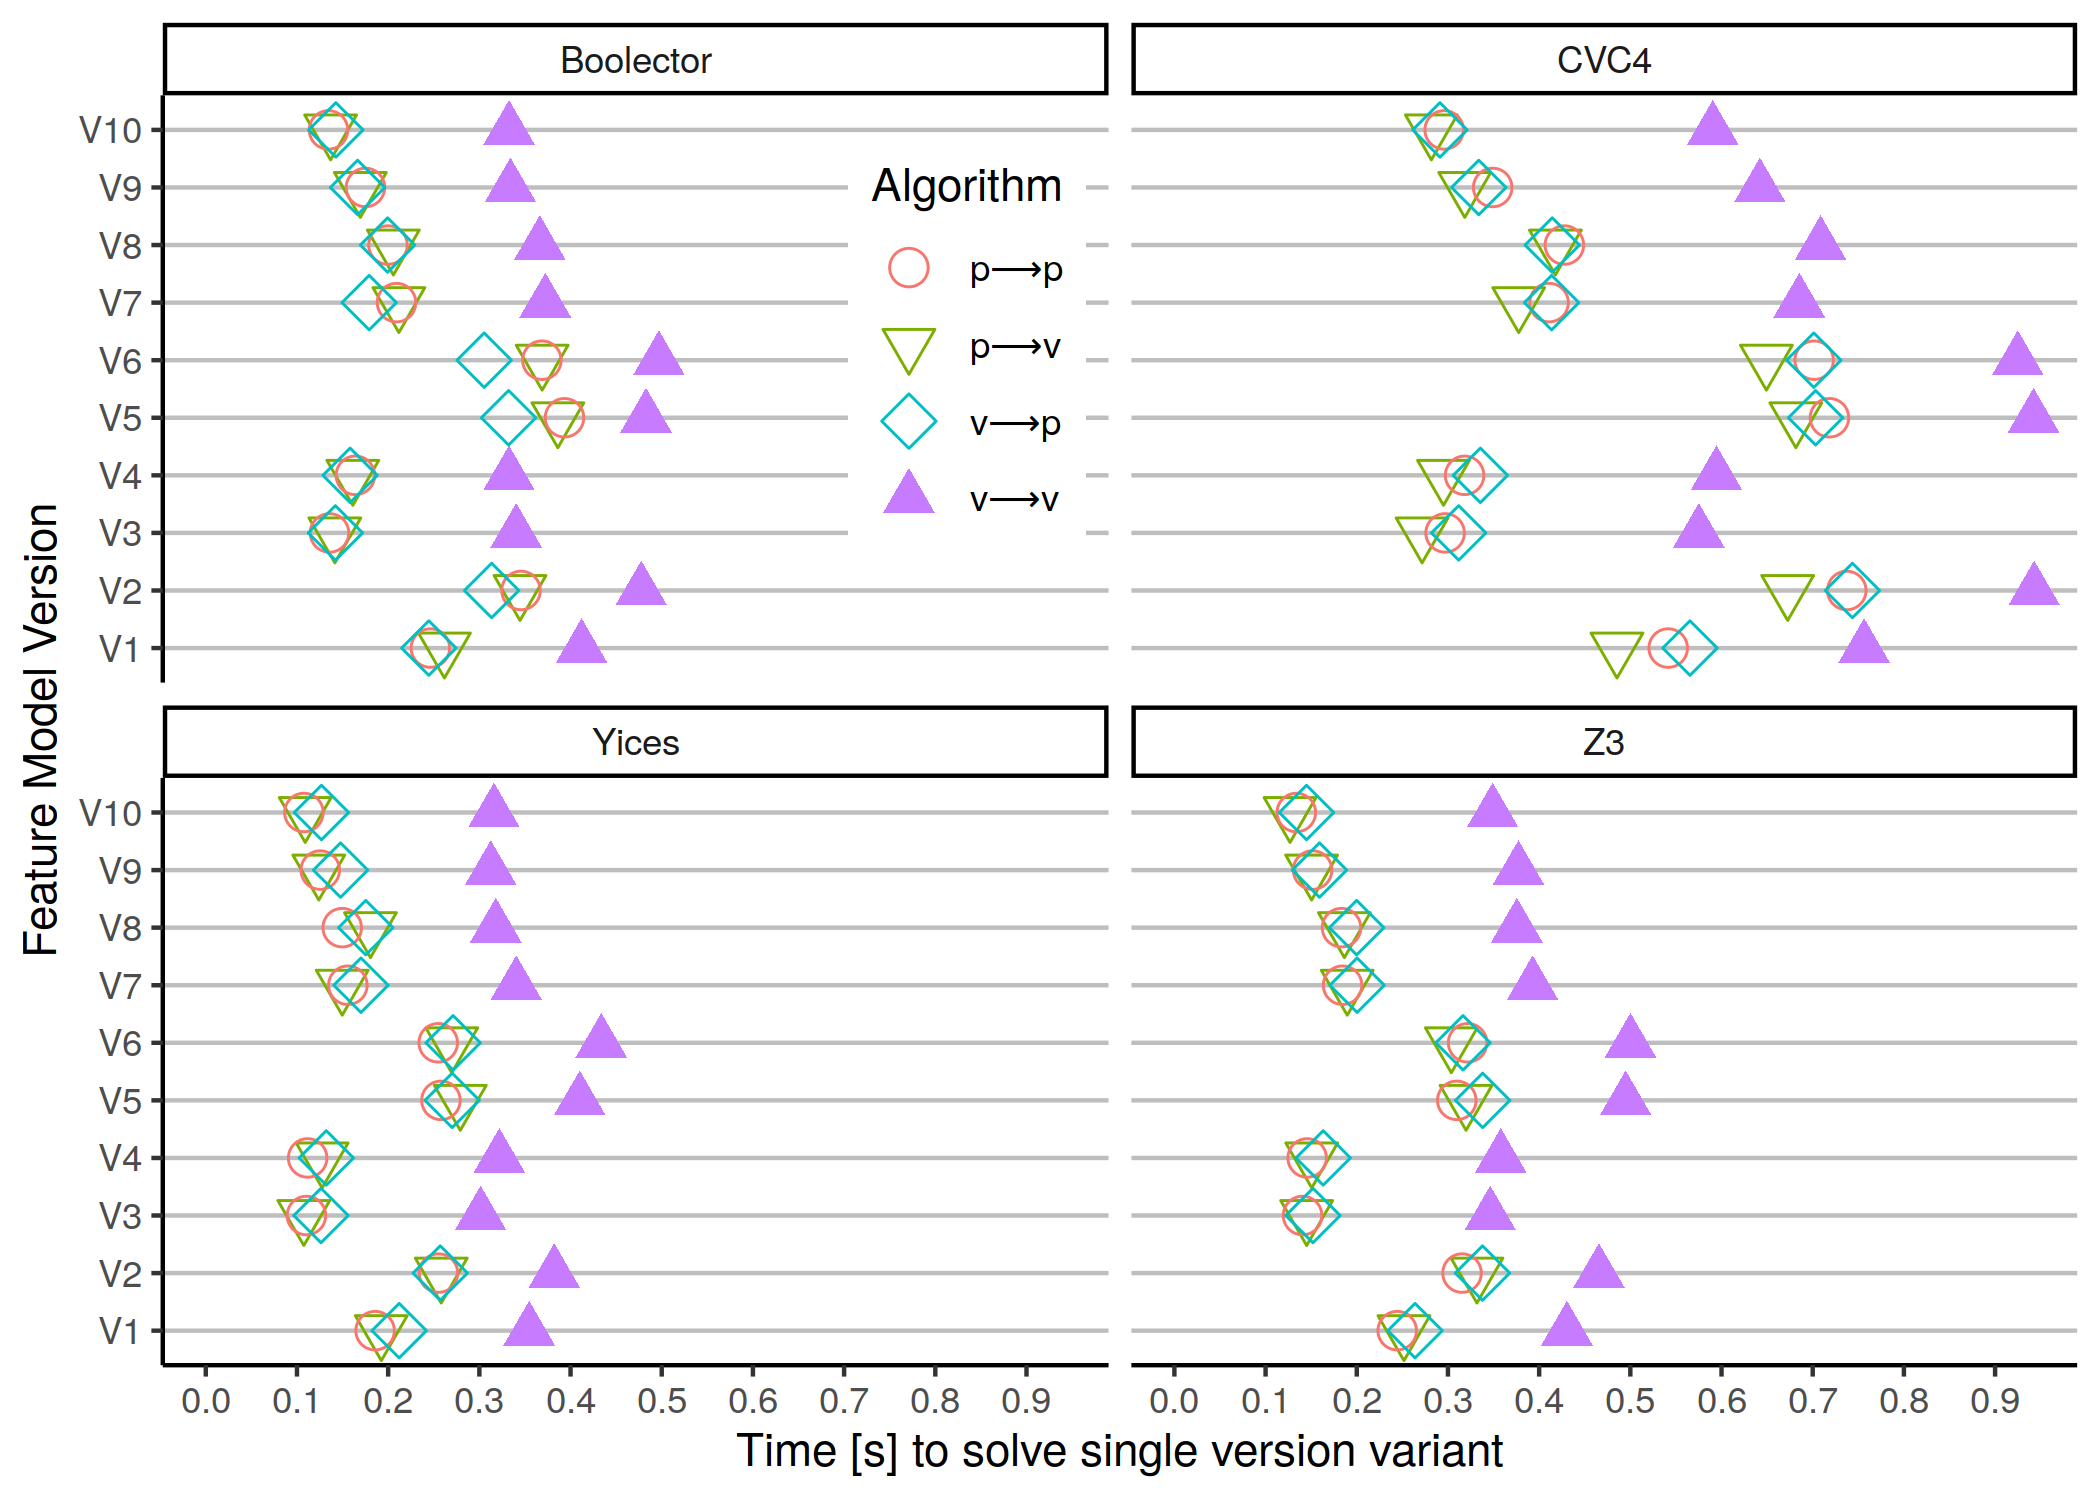
\includegraphics[width=0.95\textwidth]{Plots/RQ4_Fin}
    \caption{(Financial) RQ4: Overhead of \vTov{} on plain formulas. We observe
      that \vTov{} incurs an average slowdown of 75\% for the \fin{}
      dataset, when solving a version variant.}%
    \label{res:overhead:fin}
  \end{subfigure}
\end{figure}
%
\autoref{res:overhead:auto} and \autoref{res:overhead:fin} displays the
bootstrapped averages of each version variant, for each algorithm, and base
solver for the \auto{}, and \fin{} datasets, respectively. Given \resQ{2}, and
the composition of \fin{}, we expect \vsat{} to show slowdowns for \fin{}. This
is observed in \autoref{res:overhead:fin} and is statistically significant for
all versions. For \auto{}, only the $V_{1}$ version variant showed a significant
difference between the overhead case, \pTov{}, and \vTov{}, and between the
overhead case \pTov{}, and the typical case \vTop{}. Notably, \vTov{} did not
differ from the typical case, \vTop{}. \autoref{res:overhead:auto} suggests
statistically significant differences for other versions but omits variance,
hence the discrepancy between the plot and statistical tests. That \pTov{} was
statistically different for $V_{1}$ suggests particular formulas may not respond
well to the reduction engine, although the exact slowdown will be dependent on
the \ac{sat} problem.

\subsection{Threats to Validity}
Our results are subject to several threats to validity. Notably, we are unable
to make absolute performance claims because our study, with only two product
lines, may not be representative. To mitigate this we reused real-world data
from \nieke{}'s previous study~\citep{NMS+:GPCE18} and chose dissimilar product
lines. We inherit encoding-based threats to validity by reusing \nieke{}'s
formulas but ensured each algorithm experienced identical ordering of plain
terms as described in \autoref{section:case-studies:experimental-methodology}.

Our results and our prototype solver are based on the widely used Haskell
library sbv. While sbv is widely used it is still possibly that our performance
results are influenced by sbv and thus we inherit threats from the particulars
of the library. However, we believe this is a likely to be a common
implementation strategy for a variational solver (\ie{}, a solver built using a
library rather than a foreign function interface, similar to tools built on top
of sat4j~\citep{LP:JSAT10}) it is nonetheless a threat to validity as our
prototype directly depends on this library. To mitigate this threat we
maintained the same version of sbv throughout the experiment, employed it's
interface to interoperate for each base solver, and enforced the same code paths
through the library.

We have evinced the scalability claim with RQ1 and shown the translation and
automation of incremental solving in \autoref{chapter:vsat}. However, our
results depend on a \ac{vpl} formula as input and thus all points of variation
must be known before solving. We believe that \ac{vpl} formulas can be
incrementally and automatically constructed in practice, as new variants occur
or become known. However, assessing the challenges of \ac{vpl} construction is
left to future work, which we return to in
\autoref{section:conclusion:future-work}.

We do not provide a proof of the soundness of the prototype solver. We mitigate
this threat in several ways. We performed property-based
testing~\cite{quickcheck} on our prototype and verified that a satisfiable
variant was found to be satisfiable across all algorithms. In addition, we
define a property that ensures that for each plain model $p$, found with
\pTov{}, \vTop{}, and \pTop{}, a satisfiable model \prime*{p} was found by
substituting $p$ on the variational model returned from \vsat{}. We performed
the property-based tests with 3,000 generated \ac{vpl} formulas, finding no
counter-examples.



%%% Local Variables:
%%% mode: latex
%%% TeX-master: "../../thesis"
%%% End: